\chapter{Analysis of waveguide general approach}
In the preceding chapters, we conducted an investigation into a structural entity known as a parallel plane waveguide. This configuration encompasses two conducting boundaries, facilitating the propagation of electromagnetic energy between them in the form of distinct electric and magnetic field patterns, commonly referred to as modes. Our exploration also involved the conceptualization of electromagnetic wave propagation between these boundaries as an amalgamation of uniform plane waves.

This comprehension of modal propagation through the lens of uniform plane waves affords a comprehensive overview of how modes are established within a waveguide. Nevertheless, it is imperative to acknowledge that employing this visualization technique, which characterizes a modal pattern in terms of uniform plane wave fields, does not consistently yield the same level of simplicity that was evident in the context of the parallel plane waveguide. When dealing with structures akin to a pipe, whether they take the form of rectangular, circular, or arbitrary shapes, and the objective is to ascertain the propagation of electromagnetic energy within these structures, the process of visualizing this propagation as a superposition of uniform plane waves becomes exceedingly challenging.

As a result, we have developed a mathematical framework to address the intricacies of electromagnetic wave propagation within such structures. In this chapter, we introduce a generalized framework for the analysis of wave propagation within arbitrary waveguides. Subsequently, we endeavor to establish correlations between the mathematical outcomes derived from this framework and those obtained for the parallel plane waveguide, which we perceive as a composition of uniform plane waves. This endeavor not only enhances our confidence in the conceptualization of input currents in terms of uniform plane waves but also underscores the necessity of employing a comprehensive mathematical formulation when visualizing propagation in the absence of uniform plane waves.

Let us consider the presence of an arbitrarily configured waveguide, as depicted in Figure~\ref{fig:lect37}. In this context, we conceptualize this structure as a conducting conduit through which electromagnetic energy can traverse along the axial direction of the pipe, as exemplified by the wave propagation illustrated in the z-direction. At this juncture, we refrain from prescribing any particular shape for the cross-sectional profile; it may adopt various forms, including rectangular, circular, or any arbitrary configuration. The crucial parameter to define is the orientation of the wave, specifically in the z-direction.
\begin{figure}[h]
\centering
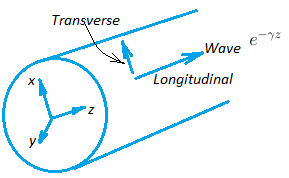
\includegraphics[width=0.7\linewidth]{/graphics/lect37}
\caption{An Arbitrarily Shaped Waveguide}
\label{fig:lect37}
\end{figure}
    
Our approach commences by establishing a comprehensive framework, originating from the Maxwell equations, to delineate the nature of the electromagnetic fields existing within this shape. Subsequently, we delve into the intricate domain of particular scenarios, specifically addressing rectangular waveguides and the propagation of modal phenomena within such waveguides. It is worth noting that any electric or magnetic field within this context can be deconstructed into two fundamental components: one aligned with the direction of wave propagation, termed the longitudinal component, and the other orthogonal to the wave propagation direction, designated as the transverse component.
\begin{align}
&\text{Electric field, }\bar{E} = \bar{E}_\bot + E_z\hat{z}\quad\text{and}\label{eqn:efieldlec37}\\
&\text{Magnetic field, }\bar{H} = \bar{H}_\bot + H_z\hat{z}\label{eqn:hfieldlec37}
\end{align}
\begin{align*}
\text{Where, }\bar{E}_\bot = E_x\hat{x} + E_y\hat{y}\text{ and }
\bar{H}_\bot = H_x\hat{x} + + H_y\hat{y}
\end{align*}
For the divergent operator, we define
\begin{equation}
\nabla = \nabla_\bot + \frac{\partial}{\partial z}\hat{z}
\label{eqn:transversegrad}
\end{equation}
\begin{align*}
\text{Where, }\nabla_\bot = \frac{\partial}{\partial x}\hat{x} + \frac{\partial}{\partial y}\hat{y}
\end{align*}
We start with Maxwell's equations\index{maxwell's equations} and substitute Equations~\ref{eqn:transversegrad},~\ref{eqn:efieldlec37} and~\ref{eqn:hfieldlec37}. Considering the Faraday's law in differential form, we have
\begin{align*}
\nabla\times\bar{E} = j\omega\mu\bar{H}
\end{align*}
\begin{dmath*}
\left[\nabla_\bot + \frac{\partial}{\partial z}\hat{z}\right]\times(\bar{E}_\bot + E_z\hat{z}) = -j\omega\mu(\bar{H}_\bot + H_z\hat{z})
\end{dmath*}
\begin{dmath*}
\nabla_\bot\times\bar{E}_\bot + \nabla_\bot\times(E_z\hat{z}) + \frac{\partial}{\partial z}\hat{z}\times\bar{E}_\bot + \frac{\partial}{\partial z}\hat{z}\times(E_z\hat{z}) = -j\omega\mu(\bar{H}_\bot + H_z\hat{z})
\end{dmath*}
Equating the transverse and longitudinal components of the equation, we have
\begin{dmath*}
-j\omega\mu\bar{H}_\bot = \nabla_\bot\times(E_z\hat{z}) + \frac{\partial}{\partial z}\hat{z}\times\bar{E}_\bot
\end{dmath*}
\begin{dmath}
\bar{H}_\bot = -\frac{1}{j\omega\mu} \left[\nabla_\bot\times(E_z\hat{z}) + \frac{\partial}{\partial z}\hat{z}\times\bar{E}_\bot\right]
\label{eqn:transversemag}
\end{dmath}
Similarly, considering Maxwell's modified Ampere's law equation, we substitute Equations~\ref{eqn:transversegrad},~\ref{eqn:efieldlec37} and~\ref{eqn:hfieldlec37} to get the general formulation for the magnetic field inside an arbitrarily shaped waveguide.
\begin{align*}
\nabla\times\bar{H} = j\omega\epsilon\bar{E}
\end{align*}
\begin{dmath*}
\left[ \nabla_\bot + \frac{\partial}{\partial z}\hat{z} \right] \times (H_\bot + H_z \hat{z}) = \jmath \omega\epsilon (E_\bot + E_z \hat{z})
\end{dmath*}
\begin{dmath*}
\nabla_\bot\times H_\bot + \nabla_\bot\times H_z \hat{z} +  \frac{\partial}{\partial z}\hat{z}\times H_\bot + \frac{\partial}{\partial z}\hat{z}\times H_z \hat{z} = \jmath \omega\epsilon (E_\bot + E_z \hat{z})
\end{dmath*}
Equating the transverse and longitudinal components of the equation.
\begin{dmath}
\bar{E}_\bot = \frac{1}{j\omega\epsilon} \left[\nabla_\bot\times H_z\hat{z} + \frac{\partial}{\partial z}\hat{z}\times\bar{H}_\bot\right]
\label{eqn:transverseele}
\end{dmath}
Substituting Equation~\ref{eqn:transversemag} into \ref{eqn:transverseele}
\begin{dmath*}
\bar{E}_\bot = \frac{1}{j\omega\epsilon} \left[\nabla_\bot\times H_z\hat{z} + \frac{\partial}{\partial z}\hat{z}\times \left( -\frac{1}{j\omega\mu} \left[\nabla_\bot\times(E_z\hat{z}) + \frac{\partial}{\partial z}\hat{z}\times\bar{E}_\bot\right] \right)\right] 
\end{dmath*}
Collecting like terms
\begin{dmath}
\omega^2\mu\epsilon\bar{E}_\bot-\frac{\partial}{\partial z}\hat{z}\times\frac{\partial}{\partial z}\hat{z}\times\bar{E}_\bot = \frac{1}{j\omega\epsilon} \left[\nabla_\bot\times H_z\hat{z} - \frac{1}{j\omega\mu}\frac{\partial}{\partial z}\hat{z}\times\nabla_\bot\times E_z \hat{z} \right]
\label{eqn:electricfieldinwg}
\end{dmath}
Recall, the identity for vector triple product\index{vector triple product} is
\begin{align*}
A\times B\times C = (\bar{A}\cdot\bar{C})\bar{B} - (\bar{A}\cdot\bar{B})\bar{C}
\end{align*}
\begin{dmath*}
\text{So, }\frac{\partial}{\partial z}\hat{z}\times\frac{\partial}{\partial z}\hat{z}\times\bar{E}_\bot = \frac{\partial}{\partial z}\hat{z}\left(\frac{\partial}{\partial z}\hat{z}\cdot\bar{E}_\bot\right)\hat{z} - \left(\frac{\partial}{\partial z}\hat{z}\cdot\frac{\partial}{\partial z}\hat{z}\right)\bar{E}_\bot = -\frac{\partial^2}{\partial z^2}\bar{E}_\bot\quad\text{where $\dfrac{\partial}{\partial z}\hat{z}\left(\dfrac{\partial}{\partial z}\hat{z}\cdot\bar{E}_\bot\right)\hat{z} = 0$}
\end{dmath*}
\begin{dmath*}
\text{And, }\frac{\partial}{\partial z}\hat{z}\times\nabla_\bot\times E_z\hat{z} = \nabla_\bot\left(\frac{\partial}{\partial z}\hat{z}.E_z\hat{z}\right) - \left(\frac{\partial}{\partial z}\hat{z}\cdot\nabla_\bot\right)E_z\hat{z} = \nabla_\bot\left(\frac{\partial E_z}{\partial z}\right)\quad\text{where $\dfrac{\partial}{\partial z}\hat{z}\cdot\nabla_\bot E_z\hat{z} = 0$}
\end{dmath*}
Substituting the above solutions in Equation~\ref{eqn:electricfieldinwg};
\begin{dmath}
\left[\omega^2\mu\epsilon\bar{E}_\bot+\frac{\partial^2}{\partial z^2}\bar{E}_\bot\right] = -j\omega\mu\nabla_\bot\times H_z\hat{z} + \nabla_\bot\left(\frac{\partial E_z}{\partial z}\right)\label{eqn:generalformulation}
\end{dmath}
In our current discourse, we have undertaken an examination of two Maxwell's equations. Employing various vector identities, we have embarked on the derivation of expressions characterizing the transverse component of the electric field in relation to the longitudinal components. This analytical endeavor stems from the fact that the waveguide under consideration serves as a conduit for wave propagation specifically along the z-direction, which represents the pivotal axis through which energy ultimately propagates.

Due to the prominence of the z-direction as the primary avenue for wave propagation, it is customary to treat the electric and magnetic field components aligned with this direction, denoted as the longitudinal components, as independent entities. Our objective is to articulate the transverse fields in terms of these longitudinal counterparts, which is precisely the accomplishment achieved thus far. Consequently, we have successfully ascertained the expression for the transverse field, denoted as $E_z$ and $H_z$, in relation to the longitudinal component.

Our focus remains steadfast on the wave propagation along the z-direction. In light of this, we assume the wave's directional behaviour conforms to the exponential expression $e^{-\gamma z}$, where $\gamma$ represents the propagation constant governing the wave's advancement in the z-direction. Essentially, this signifies that any electric or magnetic field within the structure, oriented along the z-axis, can be delineated by the functional form $e^{-\gamma z}$—a reflection of the travelling wave phenomena within the structure.

Mathematically, for a travelling wave in the z-direction,
\begin{align*}
\bar{E}, \bar{H} \sim e^{-\gamma z}\\
\text{and }\frac{\partial}{\partial z} \equiv -\gamma\\
\frac{\partial^2}{\partial z^2} \equiv \gamma^2
\end{align*}
So Equation~\ref{eqn:generalformulation} becomes;
\begin{align*}
(\omega^2\mu\epsilon + \gamma^2)\bar{E}_\bot = -j\omega\mu\nabla_\bot\times(H_z\hat{z})-\gamma\nabla_\bot E_z
\end{align*}
Let's define
\begin{align}
\omega^2\mu\epsilon + \gamma^2 \equiv h^2
\label{eqn:h}
\end{align}
we will assign some physical meaning to $h$ later. Therefore, the transverse components of electric and magnetic fields become
\begin{align}
\bar{E}_\bot = \frac{-j\omega\mu}{h^2}\nabla_\bot\times(H_z\hat{z}) - \frac{\gamma}{h^2}\nabla_\bot E_z
\label{eqn:transverseele2}
\end{align}
\begin{align}
\bar{H}_\bot = \frac{j\omega\epsilon}{h^2}\nabla_\bot\times(E_z\hat{z}) - \frac{\gamma}{h^2}\nabla_\bot H_z
\label{eqn:transversemag2}
\end{align}
The expression $\nabla_\bot\times(H_z\hat{z})$ encapsulates a curl operation within the transverse plane, while $\nabla_\bot E_z$ represents the gradient of the scalar quantity $E_z$ in the same transverse plane. Upon successfully resolving the wave propagation problem in terms of $E_z$ and $H_z$, we can subsequently deduce the corresponding fields situated within the transverse plane, denoted as $\bar{E}_\bot$ and $\bar{H}_\bot$.

The overarching methodology for addressing this problem can be outlined as follows: Initially, we select a specific geometry wherein we intend to investigate the wave propagation. Subsequently, we ascertain the solutions for $E_z$ and $H_z$ tailored to the geometry in question. Once these solutions are determined, we proceed to substitute them into the expressions for $\bar{E}_\bot$ and $\bar{H}_\bot$. This step culminates in the derivation of the individual components of the transverse fields, encompassing $E_x, E_y, H_x,$ and $H_y$.

\section{Loss-less Waveguide}
Upon examining the expressions for $\bar{E}_\bot$ and $\bar{H}_\bot$, several noteworthy observations can be made. Firstly, in the scenario where we presume that the medium under consideration is entirely devoid of losses, it follows that the quantity $\gamma$, representing the propagation constant, assumes a purely imaginary character. This arises from the fact that in a lossless medium, the wave propagates without any diminishment in its amplitude. Thus, in such cases, we establish the relationship that $\gamma$ is equivalent to $j\bar{\beta}$, with $j$ symbolizing the imaginary unit and $\bar{\beta}$ signifying the phase constant in the z-direction.
\begin{align*}
&\gamma = j\bar{\beta}\quad\text{and substituting in Equation~\ref{eqn:h}, we have}\\
&\omega^2\mu\epsilon - \bar{\beta}^2 = h^2
\end{align*}
In retrospect, if we consider the expression $\omega^2\mu\epsilon$ as the phase constant of a wave propagating through an unbounded medium, \emph{it becomes evident that the symbol $h$ in this context serves as a representation of the propagation constant specific to the transverse plane.} In essence, \emph{$h$ embodies the characteristic that quantifies how this wave propagates within the XY-plane, which is orthogonal to its primary direction of motion, thereby elucidating the wave's behavior and properties across different spatial dimensions}.

From the equations presented in Equations~\eqref{eqn:transverseele2} and~\eqref{eqn:transversemag2}, several significant insights can be gleaned. To begin with, in order for transverse fields to manifest, both $E_z$ and $H_z$ must possess non-zero values. Furthermore, even if either one of these components remains non-zero while the other is zero, transverse fields can still be established within the waveguide. This implies that the field distribution inside the waveguide can take on various configurations, including scenarios where either $E_z$ equals zero, $H_z$ equals zero, or both are non-zero.

However, it is noteworthy that when both $E_z$ and $H_z$ are set to zero, transverse fields generally cease to exist, with the exception being when the parameter $h$ equals zero. Consequently, we can derive some intriguing conclusions from this result. Specifically, for fields to sustain their presence within the structure, it is imperative that both $E_z$ and $H_z$ are non-zero, except in cases where $h$ equals zero.

The third configuration of interest arises when $E_z$ equals zero and $H_z$ equals zero. In this scenario, transverse fields can be established, provided that the propagation constant $h$ equals zero. It is worth delving deeper into the implications of the case where all three variables, namely, $E_z$, $H_z$, and $h$, are set to zero. When both $E_z$ and $H_z$ assume zero values, this signifies that the field distributions under consideration correspond to the transverse electric and transverse magnetic fields. Consequently, these field distributions must align with the characteristics of the transverse electromagnetic (TEM) field.

In summary, the key conclusions drawn from this analysis as well as the possible configurations of the field distributions are as follows:
\begin{enumerate}[(i)]
\item Both $E_z$ and $H_z$ can not be zero except when $h=0$.
\item When $h=0$, both $E_z$ and $H_z$ MUST be zero.
\end{enumerate}
\paragraph{Case 1}When $E_z$ = 0, $H_z \neq 0 \Rightarrow TE$
\paragraph{Case 2}When $E_z \neq 0, H_z = 0 \Rightarrow TM$
\paragraph{Case 3}When $E_z = H_z = 0 \Rightarrow TEM$ then $h \equiv 0$

\begin{dmath*}
\text{From Equation~\eqref{eqn:h}, the phase constant }\bar{\beta} = \sqrt{\omega^2\mu\epsilon - h^2}
\end{dmath*}
Considering the possible configurations, when both $E_z$ and $H_z$ exhibit non-zero values, it follows that the parameter $h$ cannot assume a zero value, implying that $h$ is inherently a finite quantity. In the event that $h$ equals zero, $\bar{\beta}$ assumes the form of $\omega \sqrt{\mu\epsilon}$, leading to a phase velocity that becomes independent of frequency. This observation carries significant implications. Specifically, it underscores that the TE (Transverse Electric) mode or TM (Transverse Magnetic) mode inevitably exhibits dispersion, with its velocity being a function of frequency. Conversely, the TEM (Transverse Electromagnetic) mode must inherently be non-dispersive since, in this case, the phase velocity aligns with the velocity within the medium.

Consequently, we derive two pivotal conclusions from this analysis:
\begin{enumerate}[(i)]
\item TE and TM modes are dispersive
\item TEM mode is non-dispersive
\end{enumerate}
In practical terms, this signifies that when attempting to excite field distributions, whether they manifest as transverse electric or transverse magnetic modes, their velocities will invariably vary as a function of frequency. Conversely, if we consider a mode and, if it exists, as a transverse electromagnetic mode, this mode will consistently propagate at a velocity independent of the frequency.

It is worth noting that not all structures may support the propagation of transverse electromagnetic modes. Nevertheless, when such modes are present within a structure, they exhibit the distinctive quality of non-dispersiveness and consistently travel at a velocity equal to the speed within the unbounded medium encompassed by the waveguide. By conducting this comprehensive analysis, we have arrived at these noteworthy conclusions. Subsequently, utilizing the derived expression, we can proceed to analyze the propagation characteristics of specific waveguides.

Before we take up the specific waveguide problems, let us write down these transverse fields very explicitly which are;
\begin{dmath*}
\nabla_\bot\times(\psi\hat{z}) \equiv 
\footnotemark\begin{vmatrix}
\hat{x} & \hat{y} &\hat{z}\\
\partialderivative{}{x} & \partialderivative{}{y} & 0\\
0 & 0 & \psi
\end{vmatrix} = \frac{\partial\psi}{\partial y}\hat{x} - \frac{\partial\psi}{\partial x}\hat{y}
\end{dmath*}
\footnotetext{
We assume the Cartesian coordinates here and so we can derive the transverse field components in terms of the longitudinal components.
}
Substituting this transverse gradient into Equations~\eqref{eqn:transverseele2} and~\eqref{eqn:transversemag2} considering a lossless waveguide, then the expressions essentially would be
\begin{align}
E_x = -\frac{j\omega\mu}{h^2}.\frac{\partial H_z}{\partial y} - \frac{j\bar{\beta}}{h^2}.\frac{\partial E_z}{\partial x}
\label{eqn:transverseex}\\
E_y = \frac{j\omega\mu}{h^2}.\frac{\partial H_z}{\partial x} - \frac{j\bar{\beta}}{h^2}.\frac{\partial E_z}{\partial y}
\label{eqn:transverseey}\\
H_x = \frac{j\omega\epsilon}{h^2}.\frac{\partial E_z}{\partial y} - \frac{j\bar{\beta}}{h^2}.\frac{\partial H_z}{\partial x}
\label{eqn:transversehx}\\
H_y = -\frac{j\omega\epsilon}{h^2}.\frac{\partial E_z}{\partial x} - \frac{j\bar{\beta}}{h^2}.\frac{\partial H_z}{\partial y}
\label{eqn:transversehy}
\end{align}
The expressions exhibit notable symmetry and possess a mnemonic quality, rendering them easy to commit to memory. With this comprehensive development for mode propagation within a waveguide in place, we are now equipped to explore specific instances. As we've established, two distinct types of modes can exist: the transverse electric (TE) mode and the transverse magnetic (TM) mode. We've also examined a unique case—the transverse electromagnetic (TEM) mode. 

Now, we delve into a highly specific scenario, namely, the rectangular waveguide. In this context, the waveguide's cross-sectional profile adopts a rectangular shape. This prompts an intriguing inquiry: \emph{What types of fields will propagate within this rectangular waveguide?}

\section*{Exercises}
\begin{ExerciseList}
\Exercise[label={ex371}]
What are the possible configurations of the field distributions in a waveguide?
\end{ExerciseList}
